% !TeX program = lualatex
% chktex-file 1
% chktex-file 8
% chktex-file 12
% chktex-file 26
% chktex-file 36
\documentclass[a4paper,12pt]{extarticle}

\usepackage[
  paperwidth=384bp,
  paperheight=192bp,
  left=3pt,
  right=3pt,
  top=2pt,
  bottom=1pt
]{geometry}
\usepackage{array}
\usepackage{tikz}
\usepackage{xcolor}
\usepackage{unicode-math}
\usetikzlibrary{arrows.meta,calc,positioning}

\setmainfont{Latin Modern Roman}
\setmathfont{STIXTwoMath-Regular.otf}
\setmathfont[version=bold,FakeBold=7]{STIXTwoMath-Regular.otf}

\pagenumbering{gobble}
\setlength{\parindent}{0pt}
\setlength{\parskip}{1.05pt}
\setlength{\tabcolsep}{2.4pt}
\renewcommand{\arraystretch}{1.02}
\newcolumntype{L}[1]{>{\raggedright\arraybackslash}p{#1}}
\emergencystretch=2em
\hfuzz=4pt
\hbadness=10000
\raggedright

\definecolor{Pcol}{RGB}{130,40,180}
\definecolor{RuleCol}{RGB}{25,25,25}
\definecolor{BoxBg}{RGB}{250,250,246}
\definecolor{BoxEmpty}{RGB}{255,255,255}
\definecolor{Good}{RGB}{20,130,45}
\definecolor{Warn}{RGB}{210,85,20}
\definecolor{Blue}{RGB}{35,105,200}
\definecolor{PBlue}{RGB}{35,105,200}
\definecolor{PRed}{RGB}{230,20,20}
\definecolor{distblue}{RGB}{55,115,195}

\makeatletter
\renewcommand\Large{\@setfontsize\Large{15.2pt}{9.4pt}}
\makeatother

\newcommand{\mop}[1]{\mathop{\symrm{#1}}\nolimits}
\renewcommand{\ln}{\mop{ln}}
\newcommand{\SlideHead}[2]{{\fontsize{18.1}{10.4}\selectfont\bfseries #1}\hfill{\fontsize{18.1}{10.4}\selectfont\bfseries\textcolor{Pcol}{#2}}\par}
\newcommand{\Slide}[2]{%
  \newpage
  \enlargethispage{30pt}%
  \SlideHead{#1}{#2}%
  \vspace{-1pt}\noindent\textcolor{RuleCol}{\rule{\linewidth}{0.55pt}}\par\vspace{-1pt}%
}
\newcommand{\FirstSlide}[2]{%
  \enlargethispage{30pt}%
  \SlideHead{#1}{#2}%
  \vspace{-1pt}\noindent\textcolor{RuleCol}{\rule{\linewidth}{0.55pt}}\par\vspace{-1pt}%
}
\newcommand{\DCard}[1]{%
  \vspace{0pt}\begingroup\setlength{\fboxsep}{1.05pt}%
  \fcolorbox{RuleCol}{BoxBg}{\begin{minipage}{0.985\linewidth}{\fontsize{11.2}{11.75}\selectfont\bfseries #1}\end{minipage}}\par
  \endgroup\vspace{0.7pt}%
}
\newcommand{\LargeText}[1]{{\par\noindent\fontsize{11.7}{12.2}\selectfont\ignorespaces #1\par}}
\newcommand{\MaxText}[1]{{\par\noindent\fontsize{12.25}{12.7}\selectfont\ignorespaces #1\par}}
\newcommand{\UltraText}[1]{{\par\noindent\fontsize{13.0}{13.45}\selectfont\ignorespaces #1\par}}
\newcommand{\MegaText}[1]{{\par\noindent\fontsize{13.8}{14.2}\selectfont\ignorespaces #1\par}}
\newcommand{\SmallText}[1]{{\par\noindent\fontsize{10.15}{10.65}\selectfont\ignorespaces #1\par}}
\newcommand{\TinyText}[1]{{\par\noindent\fontsize{9.15}{9.55}\selectfont\ignorespaces #1\par}}
\newcommand{\StepEq}[1]{{\fontsize{15.9}{14.2}\selectfont\[#1\]}}
\newcommand{\StepTinyEq}[1]{{\fontsize{13.35}{11.45}\selectfont\[#1\]}}
\newcommand{\StepMicroEq}[1]{{\fontsize{12.15}{10.45}\selectfont\[#1\]}}
\newcommand{\StepMaxEq}[1]{{\fontsize{18.2}{16.0}\selectfont\[#1\]}}
\newcommand{\MTTrayColumn}{%
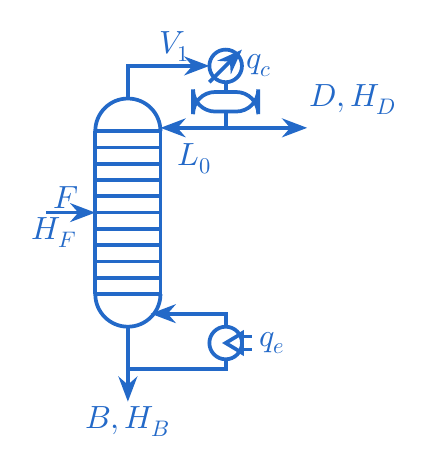
\begin{tikzpicture}[
    Blue,
    line width=1.35pt,
    >=Stealth,
    font=\sffamily\bfseries\boldmath\fontsize{28}{28}\selectfont,
    scale=0.414,
    transform shape
]
  \draw (-1,-2.5) -- (-1,2.5);
  \draw (1,-2.5) -- (1,2.5);
  \draw (1,2.5) arc (0:180:1);
  \draw (-1,-2.5) arc (180:360:1);

  \foreach \y in {-2.5,-2.0,-1.5,-1.0,-0.5,0,0.5,1.0,1.5,2.0,2.5} {
    \draw (-1,\y) -- (1,\y);
  }

  \draw[->] (-2.5,0) -- (-1,0);
  \node[anchor=south east] at (-1.5,0) {\(F\)};
  \node[anchor=north east] at (-1.5,0) {\(H_F\)};

  \draw[->] (0,3.5) -- (0,4.5) -- (2.5,4.5) node[pos=0.58,anchor=south] {\(V_1\)};
  \draw (3,4.5) circle (0.5);
  \draw[->] (2.5,4.0) -- (3.5,5.0);
  \node[anchor=west] at (3.5,4.5) {\(q_c\)};

  \draw (3,4.0) -- (3,3.7);
  \draw[rounded corners=8pt] (2.0,3.1) rectangle (4.0,3.7);

  \draw (3,3.1) -- (3,2.6);
  \draw[->] (3,2.6) -- (1,2.6) node[pos=0.47,anchor=north,yshift=-10pt] {\(L_0\)};
  \draw[->] (3,2.6) -- (5.5,2.6) node[pos=0.90,anchor=south west,xshift=5pt,yshift=8pt] {\(D,H_D\)};

  \draw (0,-3.5) -- (0,-4.8);
  \draw[->] (0,-4.8) -- (0,-5.8) node[anchor=north] {\(B,H_B\)};

  \draw (0,-4.8) -- (3,-4.8) -- (3,-4.5);
  \draw (3,-4.0) circle (0.5);
  \draw (3,-4.0) -- (3.5,-3.7) -- (3.5,-4.3) -- cycle;
  \draw (3.5,-3.8) -- (3.8,-3.8);
  \draw (3.5,-4.2) -- (3.8,-4.2);
  \node[anchor=west] at (3.9,-4.0) {\(q_e\)};

  \draw[->] (3,-3.5) -- (3,-3.1) -- (0.7,-3.1);
\end{tikzpicture}%
}
\expandafter\newcommand\csname BoxGraphic01\endcsname{\raisebox{-10pt}{\MTTrayColumn}}
\tikzset{
  mtaxis/.style={-{Latex[length=4.0pt,width=3.0pt]}, line width=0.45pt, draw=RuleCol},
  mtdiag/.style={line width=0.55pt, draw=RuleCol},
  mtwork/.style={line width=1.0pt, draw=PRed},
  mtstrip/.style={line width=1.0pt, draw=Good},
  mtfeed/.style={line width=1.0pt, draw=Pcol},
  mtstep/.style={line width=0.82pt, draw=RuleCol},
  mtlab/.style={font=\fontsize{6.2}{6.4}\selectfont\bfseries, inner sep=0.25pt},
  mtdot/.style={circle, fill=RuleCol, inner sep=0.8pt}
}
\newcommand{\MTAxes}{%
  \draw[mtaxis] (0,0) -- (1.08,0) node[mtlab,below] {$x$};
  \draw[mtaxis] (0,0) -- (0,1.08) node[mtlab,left] {$y$};
  \draw[mtdiag] (0,0) -- (1,1) node[mtlab,above right] {$y=x$};
}
\newcommand{\MTMarks}{%
  \foreach \x/\lab in {0.12/x_B,0.45/z_F,0.88/x_D}{%
    \draw[RuleCol,line width=0.3pt] (\x,0) -- (\x,-0.025) node[mtlab,below] {$\lab$};}
}
\newcommand{\MTQLinesMini}{%
\begingroup
\resizebox{0.97\linewidth}{!}{%
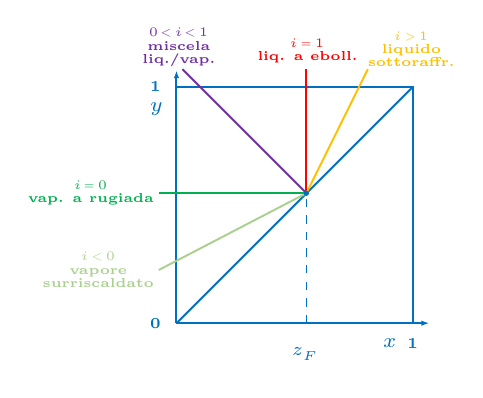
\begin{tikzpicture}[x=0.30cm,y=0.30cm,line width=0.70pt]
  \definecolor{plotblue}{RGB}{0,112,192}
  \definecolor{plotpurple}{RGB}{112,48,160}
  \definecolor{plotgreen}{RGB}{0,176,80}
  \definecolor{plotlightgreen}{RGB}{169,208,142}
  \definecolor{plotorange}{RGB}{255,192,0}
  \definecolor{plotred}{RGB}{255,0,0}
  \tikzset{qlab/.style={align=center,font=\fontsize{4.7}{4.85}\selectfont\bfseries,inner sep=0.2pt}}
  \draw[plotblue] (0,10) -- (10,10) -- (10,0);
  \draw[plotblue,-{Latex[length=2.8pt,width=2.0pt]}] (0,0) -- (10.70,0);
  \draw[plotblue,-{Latex[length=2.8pt,width=2.0pt]}] (0,0) -- (0,10.70);
  \draw[plotblue] (0,0) -- (10,10);
  \coordinate (ZF) at (5.5,5.5);
  \draw[plotblue,dashed,line width=0.4pt] (5.5,0) -- (ZF);
  \draw[plotred] (ZF) -- (5.5,10.75);
  \draw[plotorange] (ZF) -- (8.1,10.75);
  \draw[plotpurple] (ZF) -- (0.25,10.75);
  \draw[plotgreen] (ZF) -- (-0.75,5.5);
  \draw[plotlightgreen] (ZF) -- (-0.75,2.25);
  \fill[plotblue] (ZF) circle (0.95pt);
  \node[plotblue,font=\fontsize{7.4}{7.4}\selectfont\bfseries\itshape] at (-0.85,9.05) {$y$};
  \node[plotblue,font=\fontsize{7.4}{7.4}\selectfont\bfseries\itshape] at (9.05,-0.85) {$x$};
  \node[plotblue,font=\fontsize{5.5}{5.5}\selectfont\bfseries,left=2pt] at (0,0) {0};
  \node[plotblue,font=\fontsize{5.5}{5.5}\selectfont\bfseries,left=2pt] at (0,10) {1};
  \node[plotblue,font=\fontsize{5.5}{5.5}\selectfont\bfseries,below=2pt] at (10,0) {1};
  \node[plotblue,font=\fontsize{6.7}{6.7}\selectfont\bfseries\itshape,anchor=south west] at (4.5,-2) {$z_F$};
  \node[plotpurple,qlab,anchor=south] at (0.1,10.78) {$0<i<1$\\miscela\\liq./vap.};
  \node[plotred,qlab,anchor=south] at (5.55,10.95) {$i=1$\\liq. a eboll.};
  \node[plotorange,qlab,anchor=south west] at (8.05,10.78) {$i>1$\\liquido\\sottoraffr.};
  \node[plotgreen,qlab,anchor=east] at (-0.90,5.50) {$i=0$\\vap. a rugiada};
  \node[plotlightgreen,qlab,anchor=east] at (-0.90,2.25) {$i<0$\\vapore\\surriscaldato};
\end{tikzpicture}%
}%
\endgroup}
\newcommand{\MTPinchMini}{%
\begingroup
\resizebox{0.97\linewidth}{!}{%
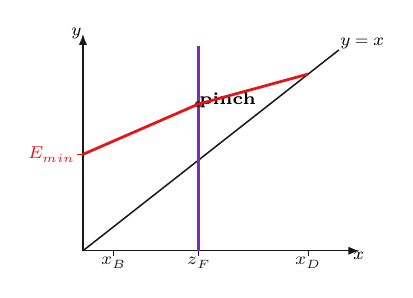
\begin{tikzpicture}[x=3.25cm,y=2.55cm]
  \MTAxes\MTMarks
  \draw[mtfeed] (0.45,0) -- (0.45,1.02);
  \node[mtdot,label={[mtlab,right]{pinch}}] at (0.45,0.73) {};
  \draw[mtwork] (0.88,0.88) -- (0.45,0.73) -- (0,0.48);
  \draw[PRed,line width=0.3pt] (0,0.48) -- (-0.025,0.48) node[mtlab,left] {$E_{min}$};
\end{tikzpicture}%
}%
\endgroup}
\newcommand{\MTCostMini}{%
\begingroup
\resizebox{0.97\linewidth}{!}{%
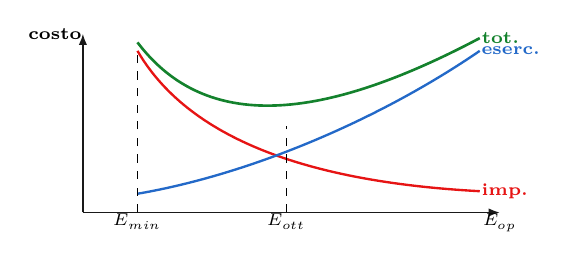
\begin{tikzpicture}[x=1.26cm,y=1.08cm]
  \draw[mtaxis] (0,0) -- (4.2,0) node[mtlab,below] {$E_{op}$};
  \draw[mtaxis] (0,0) -- (0,2.1) node[mtlab,left] {costo};
  \draw[PRed,line width=0.85pt] (0.55,1.9) .. controls (1.1,0.8) and (2.4,0.35) .. (4.0,0.25) node[mtlab,right] {imp.};
  \draw[PBlue,line width=0.85pt] (0.55,0.22) .. controls (1.7,0.45) and (3.0,1.1) .. (4.0,1.9) node[mtlab,right] {eserc.};
  \draw[Good,line width=0.95pt] (0.55,2.0) .. controls (1.2,1.0) and (2.3,1.0) .. (4.0,2.05) node[mtlab,right] {tot.};
  \draw[dashed,line width=0.35pt] (0.55,0) node[mtlab,below] {$E_{min}$} -- (0.55,1.85);
  \draw[dashed,line width=0.35pt] (2.05,0) node[mtlab,below] {$E_{ott}$} -- (2.05,1.02);
\end{tikzpicture}%
}%
\endgroup}
\newcommand{\MTStepsMini}{%
\begingroup
\resizebox{0.97\linewidth}{!}{%
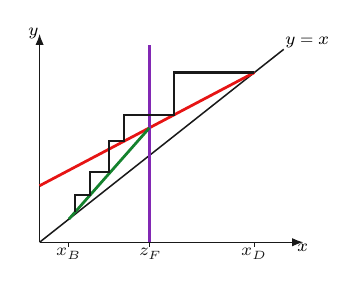
\begin{tikzpicture}[x=3.1cm,y=2.45cm]
  \MTAxes\MTMarks
  \draw[mtwork] (0,0.293) -- (0.88,0.88);
  \draw[mtfeed] (0.45,0) -- (0.45,1.02);
  \draw[mtstrip] (0.12,0.12) -- (0.45,0.593);
  \draw[mtstep] (0.88,0.88) -- (0.55,0.88) -- (0.55,0.660) --
    (0.345,0.660) -- (0.345,0.525) -- (0.285,0.525) --
    (0.285,0.363) -- (0.205,0.363) -- (0.205,0.245) --
    (0.145,0.245) -- (0.145,0.155);
\end{tikzpicture}%
}%
\endgroup}
\expandafter\newcommand\csname BoxGraphic08\endcsname{\MTQLinesMini}
\expandafter\newcommand\csname BoxGraphic10\endcsname{\MTPinchMini}
\expandafter\newcommand\csname BoxGraphic12\endcsname{\MTCostMini}
\expandafter\newcommand\csname BoxGraphic16\endcsname{\MTStepsMini}
\newcommand{\MTConversionFlow}{%
\begingroup
\resizebox{0.97\linewidth}{!}{$\displaystyle
Q_{vol}
\overset{\cdot\rho}{\underset{/\,\rho}{\rightleftharpoons}}
Q_{mass}
\overset{/\,P_m}{\underset{\cdot P_m}{\rightleftharpoons}}
Q_{mol}
\overset{/\,C}{\underset{\cdot C}{\rightleftharpoons}}
Q_{vol}
$}%
\endgroup}
\newcommand{\BoxIdea}[1]{%
  \ifcsname BoxIdea#1\endcsname
    \csname BoxIdea#1\endcsname
  \else
    idea figura\\da definire
  \fi}
\expandafter\newcommand\csname BoxIdea01\endcsname{schema colonna\\\(F,D,B\)\\con \(z_F,x_D,x_B\)}
\expandafter\newcommand\csname BoxIdea02\endcsname{flusso conversione\\massa \(\to\) moli\\\(\to x_A\)}
\expandafter\newcommand\csname BoxIdea03\endcsname{split \(F\to D+B\)\\con bilancio\\del volatile}
\expandafter\newcommand\csname BoxIdea04\endcsname{curva \(y^*(x)\)\\sopra diagonale\\+ tabella}
\expandafter\newcommand\csname BoxIdea05\endcsname{assi \(y-x\)\\diagonale\\e punti chiave}
\expandafter\newcommand\csname BoxIdea06\endcsname{CMO: \(L,V\)\\costanti sopra\\e sotto feed}
\expandafter\newcommand\csname BoxIdea07\endcsname{sezione alta\\bilancio su piatto\\e retta \(y_R\)}
\expandafter\newcommand\csname BoxIdea08\endcsname{q-line/freddezza\\con i casi\\\(i=1,0,<1,>1\)}
\expandafter\newcommand\csname BoxIdea09\endcsname{retta alta reale\\da \(x_D\)\\con \(E_{op}\)}
\expandafter\newcommand\csname BoxIdea10\endcsname{pinch: q-line\\interseca curva\\di equilibrio}
\expandafter\newcommand\csname BoxIdea11\endcsname{retta minima\\da \(x_D\)\\al pinch}
\expandafter\newcommand\csname BoxIdea12\endcsname{trade-off\\piatti vs energia\\\(E_{min}\to E_{ott}\)}
\expandafter\newcommand\csname BoxIdea13\endcsname{punto \(P\):\\incrocio \(y_R\)\\e q-line}
\expandafter\newcommand\csname BoxIdea14\endcsname{retta bassa\\per \(P\)\\e \((x_B,x_B)\)}
\expandafter\newcommand\csname BoxIdea15\endcsname{flussi interni\\\(L,V,\bar L,\bar V\)\\sopra/sotto feed}
\expandafter\newcommand\csname BoxIdea16\endcsname{gradino tipo:\\curva poi retta\\con frecce}
\expandafter\newcommand\csname BoxIdea17\endcsname{gradini numerati\\feed tray\\e ultimo fraz.}
\expandafter\newcommand\csname BoxIdea18\endcsname{ribollitore\\come stadio\\non piatto fisico}
\expandafter\newcommand\csname BoxIdea19\endcsname{riflusso totale:\\diagonale\\e \(N_{min}\)}
\expandafter\newcommand\csname BoxIdea20\endcsname{condensatore\\ribollitore\\e \(q_c,q_e\)}
\expandafter\newcommand\csname BoxIdea21\endcsname{tabella iterativa\\\(y_k\to x_k\)\\\(\to y_{k+1}\)}
\expandafter\newcommand\csname BoxIdea22\endcsname{checklist errori\\con simboli\\di attenzione}
\expandafter\newcommand\csname BoxIdeafinale\endcsname{grafico completo\\curve, rette\\e gradini}
\newcommand{\StepBoxDim}[2]{%
  \begingroup\setlength{\fboxsep}{0pt}%
  \ifcsname BoxGraphic#1\endcsname
    \begin{minipage}[c][#2][c]{#2}
      \centering
      \csname BoxGraphic#1\endcsname
    \end{minipage}%
  \else
    \fcolorbox{RuleCol}{BoxEmpty}{%
    \begin{minipage}[c][#2][c]{#2}
      \centering
      {\fontsize{12.4}{12.6}\selectfont\bfseries BOX #1}\par\vspace{3pt}
      {\fontsize{7.7}{8.0}\selectfont\bfseries\BoxIdea{#1}}
    \end{minipage}}%
  \fi
  \endgroup}
\newcommand{\StepBox}[1]{\StepBoxDim{#1}{124pt}}
\newcommand{\StepSlideFlex}[8]{%
  \Slide{#1}{#2}%
  \noindent\begin{minipage}[t]{#3\linewidth}
    #6
  \end{minipage}\hfill
  \begin{minipage}[t]{#4\linewidth}
    \vspace{0pt}\centering\StepBoxDim{#7}{#5}\par\vspace{1pt}
    \ifcsname BoxGraphic#7\endcsname\else
      {\fontsize{8.2}{8.45}\selectfont\bfseries #8}
    \fi
  \end{minipage}%
}
\newcommand{\StepSlide}[5]{\StepSlideFlex{#1}{#2}{0.615}{0.370}{134pt}{#3}{#4}{#5}}
\newcommand{\StepSlideS}[5]{\StepSlideFlex{#1}{#2}{0.615}{0.370}{134pt}{#3}{#4}{#5}}
\newcommand{\StepSlideM}[5]{\StepSlideFlex{#1}{#2}{0.615}{0.370}{134pt}{#3}{#4}{#5}}
\newcommand{\StepSlideT}[5]{\StepSlideFlex{#1}{#2}{0.615}{0.370}{134pt}{#3}{#4}{#5}}
\newcommand{\OkCheck}[1]{\textcolor{Good}{\bfseries Check:} #1}
\newcommand{\Warn}[1]{\textcolor{Warn}{\bfseries Att.:} #1}
\newcommand{\Ystar}{\textcolor{Blue}{\boldsymbol{y^{\ast}}}}
\newcommand{\BlueYStar}{\(\Ystar\)}

\begin{document}
\fontsize{17.6}{10.8}\selectfont
\mathversion{bold}
\setlength{\abovedisplayskip}{0.7pt}
\setlength{\belowdisplayskip}{0.7pt}
\setlength{\abovedisplayshortskip}{0pt}
\setlength{\belowdisplayshortskip}{0pt}
\setlength{\jot}{0.75pt}

\FirstSlide{McCabe--Thiele}{sviluppo universale}
\DCard{Ogni passaggio ha un box quadrato vuoto: poi mi dici se inserirci figura, screenshot, schema TikZ o esempio numerico.}
\StepTinyEq{\boxed{x=\text{liquido}}\qquad\boxed{y=\text{vapore}}\qquad\boxed{q=i}\qquad\boxed{R=E=L_0/D}}
\TinyText{%
\renewcommand{\arraystretch}{1.18}%
\begin{tabular}{L{0.142\linewidth}L{0.840\linewidth}}
\textbf{Scopo} & costruire rette operative, gradini e conteggio piatti/stadi per qualunque esercizio binario. \\
\textbf{Regola} & prima dati coerenti e \BlueYStar; poi q-line; poi retta alta; poi retta bassa; infine gradini. \\
\textbf{Caso chiave} & se il riflusso non è dato: calcola \(E_{min}\) dal pinch, poi scegli \(E_{op}>E_{min}\). \\
\textbf{Output} & \(D,B,L,V,\bar L,\bar V\), rette, \(N_{teorico}\), eventuali piatti reali e utility. \\
\end{tabular}}
\vspace{1pt}
\DCard{BOX Mappa: qui inserirò una panoramica generale quando mi dirai se preferisci immagine, TikZ o esempio numerico.}

\StepSlide{01. Dati}{convenzioni}{%
\DCard{Scegli il componente più volatile e usa sempre frazioni molari. Scrivi subito cosa è noto e cosa è richiesto.}
\StepMicroEq{\boxed{x_D>z_F>x_B}\quad\boxed{x=\text{liquido}}\quad\boxed{y=\text{vapore}}}
\begingroup
\renewcommand{\arraystretch}{1.16}%
{\fontsize{13.35}{14.25}\selectfont
\begin{tabular}{L{0.28\linewidth}L{0.65\linewidth}}
\textbf{Noti} & \BlueYStar/\(\alpha\), \(F,z_F,H_F,x_D,x_B\), \(E_{op}\), \(\eta\), utility. \\
\textbf{Sinonimi} & \(q=i\); \(R=E\); \(R_{min}=E_{min}\); \(R_{op}=E_{op}=E_{ott}\). \\
\textbf{Richieste} & stadi/piatti, feed tray, portate, calori, \(E_{min}\). \\
\end{tabular}}\par
\endgroup
}{01}{dati iniziali}

\Slide{02. Conversioni}{base molare}
\begingroup\setlength{\fboxsep}{0pt}%
\fcolorbox{RuleCol}{BoxBg}{%
  \begin{minipage}{0.985\linewidth}
  {\fontsize{11.5}{12.0}\selectfont\bfseries
  Se il testo dà percentuali massiche, volumetriche, kg/h o m\(^3\)/h, converti prima: McCabe lavora su moli e frazioni molari.}
  \end{minipage}}\par
\endgroup
\vspace{0pt}
\noindent\centering\resizebox{0.50\linewidth}{!}{$\displaystyle
Q_{vol}
\overset{\cdot\rho}{\underset{/\,\rho}{\rightleftharpoons}}
Q_{mass}
\overset{/\,P_m}{\underset{\cdot P_m}{\rightleftharpoons}}
Q_{mol}
\overset{/\,C}{\underset{\cdot C}{\rightleftharpoons}}
Q_{vol}
$}\par
\vspace{0pt}
\noindent\centering\resizebox{0.95\linewidth}{!}{%
{\fontsize{15.5}{16.0}\selectfont$\displaystyle
\boxed{x_A=\frac{w_A/M_A}{w_A/M_A+w_B/M_B}}
\qquad
\boxed{\dot n=\frac{\dot m}{\sum_i x_iM_i}}
$%
}}\par
\vspace{0pt}
{\par\noindent\fontsize{14.0}{14.5}\selectfont
\OkCheck{composizioni del più volatile.}\quad
\textcolor{Warn}{\bfseries !} non mescolare \% peso, \% volume e frazioni molari.\par}

\StepSlide{03. Bilanci}{D e B}{%
\DCard{Chiudi i bilanci globali prima del grafico se servono portate o carichi termici.}
\StepEq{\boxed{F=D+B}}
\StepTinyEq{\boxed{Fz_F=Dx_D+Bx_B}}
\StepTinyEq{\boxed{D=F\frac{z_F-x_B}{x_D-x_B}}}
\StepTinyEq{\boxed{B=F\frac{x_D-z_F}{x_D-x_B}}}
}{03}{bilanci}

\StepSlideS{04. Equilibrio}{curva \BlueYStar}{%
\DCard{Equilibrio \(\Ystar=f(x)\): da tabella/curva oppure da \(\alpha\).}
\StepMicroEq{\boxed{\Ystar(x)=\frac{\alpha x}{1+(\alpha-1)x}}}\vspace{-3pt}
\StepMicroEq{\boxed{x=\frac{y}{\alpha-y(\alpha-1)}}}
\TinyText{Tabella \BlueYStar:}\vspace{-8pt}
{\fontsize{9.4}{8.3}\selectfont
\[
\begin{gathered}
\boxed{y=y_1+\frac{y_2-y_1}{x_2-x_1}(x-x_1)}\\[-2pt]
\boxed{x=x_1+\frac{x_2-x_1}{y_2-y_1}(y-y_1)}
\end{gathered}
\]}
}{04}{curva eq.}

\StepSlide{05. Piano}{grafico \(y-x\)}{%
\DCard{Imposta assi \(0\)-\(1\) con stessa scala; disegna curva di equilibrio e diagonale \(y=x\).}
\StepTinyEq{\boxed{(x_D,x_D)}\quad\boxed{(z_F,z_F)}\quad\boxed{(x_B,x_B)}}
\MegaText{\OkCheck{curva sopra diagonale; estremi esclusi.}\par Segna \(x_D,z_F,x_B\): riferimenti per le rette.}
}{05}{assi e diagonale}

\StepSlide{06. Ipotesi}{CMO}{%
\DCard{Con overflow molare costante, \(L,V\) restano costanti in ciascuna sezione e le rette operative sono lineari.}
\StepEq{\boxed{q_n\simeq q_{n+1}\simeq0}}
\StepEq{\boxed{\Delta h_L\ll\lambda}}
\StepTinyEq{\boxed{\lambda\simeq\text{cost.}}\Rightarrow\boxed{L,V\text{ costanti}}}
\MaxText{Se CMO non vale, il metodo grafico semplice non basta: servono bilanci entalpici/McCabe entalpico o Ponchon--Savarit.}
}{06}{ipotesi}

\StepSlideS{07. Arricchimento}{retta alta}{%
\DCard{Sviluppo dal bilancio sulla parte sopra il piatto \(n\): vapore che sale = liquido che scende + distillato.}
\StepMicroEq{\boxed{Vy_{n+1}=Lx_n+Dx_D}\quad\boxed{E_{op}=\frac{L_0}{D}}\quad\boxed{L=L_0}}
\StepEq{\boxed{y_R=\frac{E_{op}}{E_{op}+1}x+\frac{x_D}{E_{op}+1}}}
\vspace{1.2pt}
{\par\noindent\hspace*{-1.2pt}\fontsize{14.6}{15.0}\selectfont Da \((x_D,x_D)\): \(b=x_D/(E_{op}+1)\).\par}
}{07}{retta alta}

\StepSlide{08. Feed}{q-line/i-line}{%
\DCard{La retta di alimentazione rappresenta lo stato termico del feed e passa sempre per \((z_F,z_F)\).}
\StepTinyEq{\boxed{y_F=\frac{i}{i-1}x-\frac{z_F}{i-1}}}\vspace{-2pt}
\StepTinyEq{\boxed{i=\frac{H_V-H_F}{H_V-H_L}}}
\UltraText{\(i=1\): vert. \(x=z_F\); \(i=0\): orizz. \(y=z_F\).\par
\(0<i<1\): pend. neg.; \(i>1\): sottoraffr.; \(i<0\): surrisc.}
}{08}{q-line}

\StepSlide{09. Se \(E\) dato}{via diretta}{%
\DCard{Se il rapporto di riflusso operativo è già dato, non calcolare il minimo: costruisci subito la retta alta reale.}
\StepEq{\boxed{m_R=\frac{E_{op}}{E_{op}+1}}\qquad\boxed{b_R=\frac{x_D}{E_{op}+1}}}
\StepEq{\boxed{y_R=m_Rx+b_R}}
\MegaText{Poi trova \(P=y_R\cap y_F\).\par Per \(i=1\): \(x_P=z_F\), \(y_P=y_R(z_F)\).}
}{09}{riflusso dato}

\StepSlide{10. Se \(E\) manca}{pinch}{%
\DCard{Se il riflusso non è dato, prima trovi il pinch: intersezione fra q-line e curva di equilibrio.}
\StepTinyEq{\boxed{\text{pinch }(x_p,y_p):\quad \Ystar(x_p)=y_F(x_p)}}
\StepTinyEq{\boxed{i=1:\ x_p=z_F,\ y_p=\Ystar(z_F)}}\vspace{-2pt}
\StepTinyEq{\boxed{i=0:\ y_p=z_F,\ x_p=(\Ystar)^{-1}(z_F)}}
\UltraText{Al pinch la forza motrice grafica è nulla:\par servirebbero infiniti piatti.}
}{10}{pinch}

\StepSlideS{11. Riflusso minimo}{\(E_{min}\)}{%
\DCard{La retta minima passa per \((x_D,x_D)\) e per il pinch. Serve solo a calcolare il limite.}
\StepMicroEq{\boxed{m_{min}=\frac{y_p-x_D}{x_p-x_D}}\quad\boxed{E_{min}=\frac{m_{min}}{1-m_{min}}}}
\StepTinyEq{\boxed{b_{min}=x_D-m_{min}x_D=\frac{x_D}{E_{min}+1}}}
\LargeText{\Warn{non fare i gradini sulla retta minima, a meno che il problema chieda solo il limite.}}
}{11}{retta minima}

\StepSlide{12. Riflusso operativo}{scelta}{%
\DCard{Scegli o leggi il rapporto operativo: deve essere maggiore del minimo, poi ricostruisci la retta alta.}
\StepEq{\boxed{E_{op}>E_{min}}}
\StepEq{\boxed{y_R=\frac{E_{op}}{E_{op}+1}x+\frac{x_D}{E_{op}+1}}}
\MaxText{Scelta: \(E_{op}=kE_{min}\) o \(E_{ott}\).\par Vicino a \(E_{min}\): molti piatti. Alto \(E\): più energia.}
}{12}{E operativo}

\StepSlide{13. Punto cambio}{\(P\)}{%
\DCard{Il punto operativo di cambio retta è l'intersezione fra retta alta reale e q-line.}
\StepEq{\boxed{x_P=\frac{b_F-b_R}{m_R-m_F}}}
\StepEq{\boxed{y_P=m_Rx_P+b_R}}
\StepTinyEq{\boxed{i=1:\quad x_P=z_F,\quad y_P=y_R(z_F)}}
\UltraText{\textcolor{Warn}{\bfseries !} \(P\) operativo non è sempre il pinch:\par coincide solo a riflusso minimo.}
}{13}{punto P}

\StepSlideFlex{14. Esaurimento}{retta bassa}{0.615}{0.370}{134pt}{%
\DCard{La retta di esaurimento passa per \((x_B,x_B)\) e per il punto \(P\).}
\StepTinyEq{\boxed{\bar Lx_{m-1}=\bar Vy_m+Bx_B}}\vspace{-2pt}
\StepMicroEq{\boxed{y_S=\frac{\bar L}{\bar V}x-\frac{B}{\bar V}x_B}\quad\boxed{m_S=\frac{y_P-x_B}{x_P-x_B}}}
\StepTinyEq{\boxed{y_S=m_S(x-x_B)+x_B}}
\UltraText{Forma grafica: non calcolare subito \(\bar L/\bar V\).}
}{14}{retta bassa}

\StepSlide{15. Portate interne}{sopra/sotto feed}{%
\DCard{Se l'esercizio chiede portate interne, calcolale dopo aver noto \(D\), \(E_{op}\) e \(i\).}
\StepEq{\boxed{L=L_0=E_{op}D}}
\StepEq{\boxed{V=L+D=D(E_{op}+1)}}
\StepTinyEq{\boxed{\bar L=L+iF}\qquad\boxed{\bar V=V+(i-1)F}}
\MegaText{Barra \(\bar L,\bar V\): sotto alimentazione.}
}{15}{portate}

\StepSlide{16. Gradini}{costruzione}{%
\DCard{Parti da \((x_D,x_D)\). Ogni piatto: orizzontale fino alla curva di equilibrio, verticale fino alla retta operativa.}
\StepTinyEq{\boxed{y_k\xrightarrow{\text{curva}}x_k}\qquad\boxed{x_k\xrightarrow{\text{retta}}y_{k+1}}}
\MegaText{Sopra feed usa \(y_R\); sotto feed usa \(y_S\).\par Cambia retta solo al feed.}
}{16}{scalini}

\StepSlideS{17. Conteggio}{piatti/stadi}{%
\DCard{Un tratto orizzontale che arriva alla curva di equilibrio conta uno stadio teorico. Fermati a \(x_B\).}
\StepTinyEq{\boxed{N_{teorico}=\text{numero di gradini}}}\vspace{-2pt}
\StepTinyEq{\boxed{N_{reali}\simeq\frac{N_{teorici}}{\eta}}}
\StepMicroEq{\boxed{f_{ult}\simeq\frac{x_{prec}-x_B}{x_{prec}-x_{succ}}}\qquad\boxed{N=N_{interi}+f_{ult}}}
\vspace{1.0pt}
\UltraText{Piatti installati: arrotonda per eccesso.}
}{17}{conteggio}

\StepSlide{18. Ribollitore}{convenzioni}{%
\DCard{Il ribollitore totale si comporta come uno stadio di equilibrio, ma spesso non è un piatto fisico.}
\StepEq{\boxed{\text{ribollitore totale}\approx1\text{ stadio}}}
\StepEq{\boxed{N_{piatti}=N_{stadi}-1}}
\vspace{1.2pt}
\MaxText{Sottrai 1 solo se il testo include il ribollitore negli stadi.}
}{18}{reboiler}

\StepSlide{19. Limite totale}{Fenske}{%
\begingroup\setlength{\fboxsep}{1.15pt}%
\fcolorbox{RuleCol}{BoxBg}{\begin{minipage}{0.985\linewidth}{\fontsize{12.2}{12.85}\selectfont\bfseries A riflusso totale le rette operative coincidono con la diagonale; il numero di stadi è minimo.}\end{minipage}}\par
\endgroup\vspace{1.4pt}
\StepEq{\boxed{E_{op}\to\infty\Rightarrow y=x}\qquad\boxed{N=N_{min}}}
\vspace{1.0pt}
\StepTinyEq{\boxed{N_{min}=\frac{\ln\!\left[\dfrac{x_D}{1-x_D}\dfrac{1-x_B}{x_B}\right]}{\ln\alpha}}}
\vspace{1.0pt}
\MegaText{Binaria con \(\alpha\) circa costante. Limite, non esercizio operativo.}
}{19}{Fenske}

\StepSlide{20. Energia}{utility}{%
\DCard{Se sono richiesti condensatore, ribollitore, acqua o vapore di servizio, usa portate interne e bilancio energetico.}
\StepEq{\boxed{V_1=D(E_{op}+1)}}
\StepEq{\boxed{q_c=V_1\lambda}}
\StepTinyEq{\boxed{FH_F+q_e=q_c+DH_D+BH_B}}\vspace{-2pt}
\StepTinyEq{\boxed{\dot m_{cw}=\frac{q_c}{c_p\Delta T}}}
}{20}{energia}

\StepSlide{21. Calcolatrice}{tabella scalini}{%
\DCard{Senza disegno preciso: tabella iterativa, equilibrio inverso poi retta operativa.}
\begingroup
\renewcommand{\arraystretch}{1.14}%
{\fontsize{14.1}{15.2}\selectfont
\begin{tabular}{L{0.09\linewidth}L{0.19\linewidth}L{0.19\linewidth}L{0.17\linewidth}L{0.18\linewidth}}
\textbf{k} & \textbf{\(y_k\)} & \textbf{\(x_k\)} & \textbf{retta} & \textbf{next} \\
1 & \(x_D\) & \((\Ystar)^{-1}\) & \(R/S\) & \(y_{op}\) \\
2 & \(y_2\) & \((\Ystar)^{-1}\) & \(R/S\) & \(y_{op}\) \\
\(k\) & \(y_k\) & \(x_k\) & \(R\to S\) & \(y_{k+1}\) \\
\end{tabular}}\par
\endgroup
\vspace{1.2pt}
\StepTinyEq{\boxed{x_k=(\Ystar)^{-1}(y_k)}\qquad\boxed{y_{k+1}=y_{op}(x_k)}}
\vspace{0.8pt}
\MegaText{Cambia da \(R\) a \(S\) solo al feed.}
}{21}{tabella}

\StepSlide{22. Anti-errori}{check finale}{%
\DCard{Check finale: errori più frequenti negli esercizi.}
\LargeText{%
\begin{tabular}{L{0.26\linewidth}L{0.65\linewidth}}
\textbf{Compos.} & frazioni molari volatile; non \% peso. \\
\textbf{Equil.} & curva sopra diagonale; interpola se tabella. \\
\textbf{Rette} & \(y_R\) passa da \((x_D,x_D)\); \(y_S\) da \((x_B,x_B)\) e \(P\). \\
\textbf{Minimo} & \(E_{min}\) non è retta operativa; usa\\[-1pt]
& \(E_{op}>E_{min}\). \\
\textbf{Conteggio} & orizz.=stadio; ribollitore secondo convenzione. \\
\end{tabular}}
}{22}{controlli}

\Slide{Schema rapido}{da copiare}
\noindent\begin{minipage}[t]{0.58\linewidth}
\TinyText{%
\begin{tabular}{L{0.10\linewidth}L{0.78\linewidth}}
1 & converti dati e chiudi bilanci \(D,B\) \\
2 & costruisci \(\Ystar(x)\): tabella, \(\alpha\), \BlueYStar \\
3 & disegna diagonale e segna \(x_D,z_F,x_B\) \\
4 & traccia q-line/i-line da \((z_F,z_F)\) \\
5 & se \(E\) manca: pinch \(\to E_{min}\to E_{op}\) \\
6 & retta alta operativa \(y_R\), poi \(P=y_R\cap y_F\) \\
7 & retta bassa per \(P\) e \((x_B,x_B)\) \\
8 & gradini curva/retta, cambio al feed, conta fino a \(x_B\) \\
9 & correggi per frazione ultimo piatto, efficienza, ribollitore \\
10 & se richiesto: portate interne e bilanci energia \\
\end{tabular}}
\end{minipage}\hfill
\begin{minipage}[t]{0.335\linewidth}
\centering\StepBox{finale}\par\vspace{1pt}
{\fontsize{8.2}{8.45}\selectfont\bfseries schema completo}
\end{minipage}
\DCard{Dimmi per ogni BOX cosa vuoi: immagine del grafico, mini-schema TikZ, screenshot calcolatrice, curva reale o esempio numerico.}

\end{document}
